\section{Experimental Design} \label{experiment design}

In order to evaluate the efficacy of schemes presented in
Section~\ref{design}, we have performed experiments for seven benchmarks
on three architectures. This section describes the
setup used in our experiments.

\subsection{Systems and Benchmarks}

We conducted our experiments on three platforms: AMD Opteron, Intel Sandy Bridge,
and Intel Broadwell.  The architectural
details for these systems are provided in \Cref{settings}.
Our benchmark suite (see \Cref{table:apps}) consists of seven
HPC programs: AMG~\cite{amg2013}, LULESH
\cite{LULESH}, Cloverleaf (CL)~\cite{cloverleaf}, 351.bwaves, 362.fma3d,
363.swim~\cite{specomp2012} and Optewe~\cite{sc2017}.  Three of these benchmarks (bwaves, fma3d, and
swim) are from the SPEC OMP 2012 suite, while the rest are widely used HPC
proxy applications.  These benchmarks have been
selected based on two criteria.  First, they are written in different
languages and exploit multi-core parallelism suitable for HPC via
OpenMP pragmas.  Second, they feature more than one hot loop, which
resembles realistic applications (unlike many other benchmarks with
just a single hot loop). While multiple hot loops present difficulties
for the compiler in coordinating various loop optimizations,
they also provide opportunity to optimize different parts of the code differently.
%
%dvfs, dct
%Benchmark description
%Input selection
% We also report standard deviations in \Cref{table:stdB},
% \Cref{table:stdS} and \Cref{table:stdO}.

All our experiments have been run on CentOS Linux 7.3.1611 and the benchmarks
were compiled
with the Intel C/C++ Compiler 17.04. OpenMP thread placement has been set to
``fine, proclist=[...] explicit'', where proclist is specified in \Cref{settings}.
%
Details of the OpenMP configurations are presented in \Cref{settings}.
Scientific codes follow a time-step execution pattern repeatedly
performing approximations with decreasing numerical error in an outer
loop. Hence, we only run for a small number of time-steps (seconds)
and then exit prematurely once we have obtained a stable execution
time for a time-step. Any optimization then scales up to a full run
over all time-steps (hours). To this end, input sizes and time-steps
(iteration counts of simulation outer loop) have been adjusted so that
every single run is less than 30 seconds for O3 baseline
compilation. In the first experiments (\Cref{cv sensitivity}, ~\Cref{overallResults} and ~\Cref{beatPGO}), we use the same inputs for
tuning and testing; in later experiments, we evaluate the impact of
different inputs (\Cref{inputsensitivity}).

\begin{comment}
Note that 
To account for run-to-run variability, each code variant is executed
10 times and their average is presented as the representative runtime.
\end{comment}

\begin {table}[t]
%\nocaptionrule
\caption{List of benchmarks. LOC: lines of source code.}
\vspace{-2mm}
\centering
{\footnotesize
\label{table:apps}
\begin{tabular}{ p{2.5cm}p{2cm}p{1cm}p{7.1cm}}
%\hline
%  & \\
\textbf{Name} & \textbf{Language} & \textbf{LOC} &  \textbf{ Domain} \\
\hline
AMG & C & 113k & Math: linear solver \\ \hline
LULESH & C++ & 7.2k & Hydrodynamics \\ \hline
Cloverleaf (CL) & C, Fortran & 14.5k & Hydrodynamics\\ \hline
351.bwaves & Fortran& 1.2k & Computational fluid dynamics, SPEC OMP 2012 \\ \hline
362.fma3d & Fortran& 62k & Mechanical response simulation, SPEC OMP 2012 \\ \hline
363.swim & Fortran& 0.5k & Weather prediction, SPEC OMP 2012 \\ \hline
Optewe & C++& 2.7k & Seismic wave simulation \\ \hline
\end{tabular}
}
\end {table}


% why LULESH on Opteron does not bring any performance benefit?
\begin{comment}

\begin{figure*}
%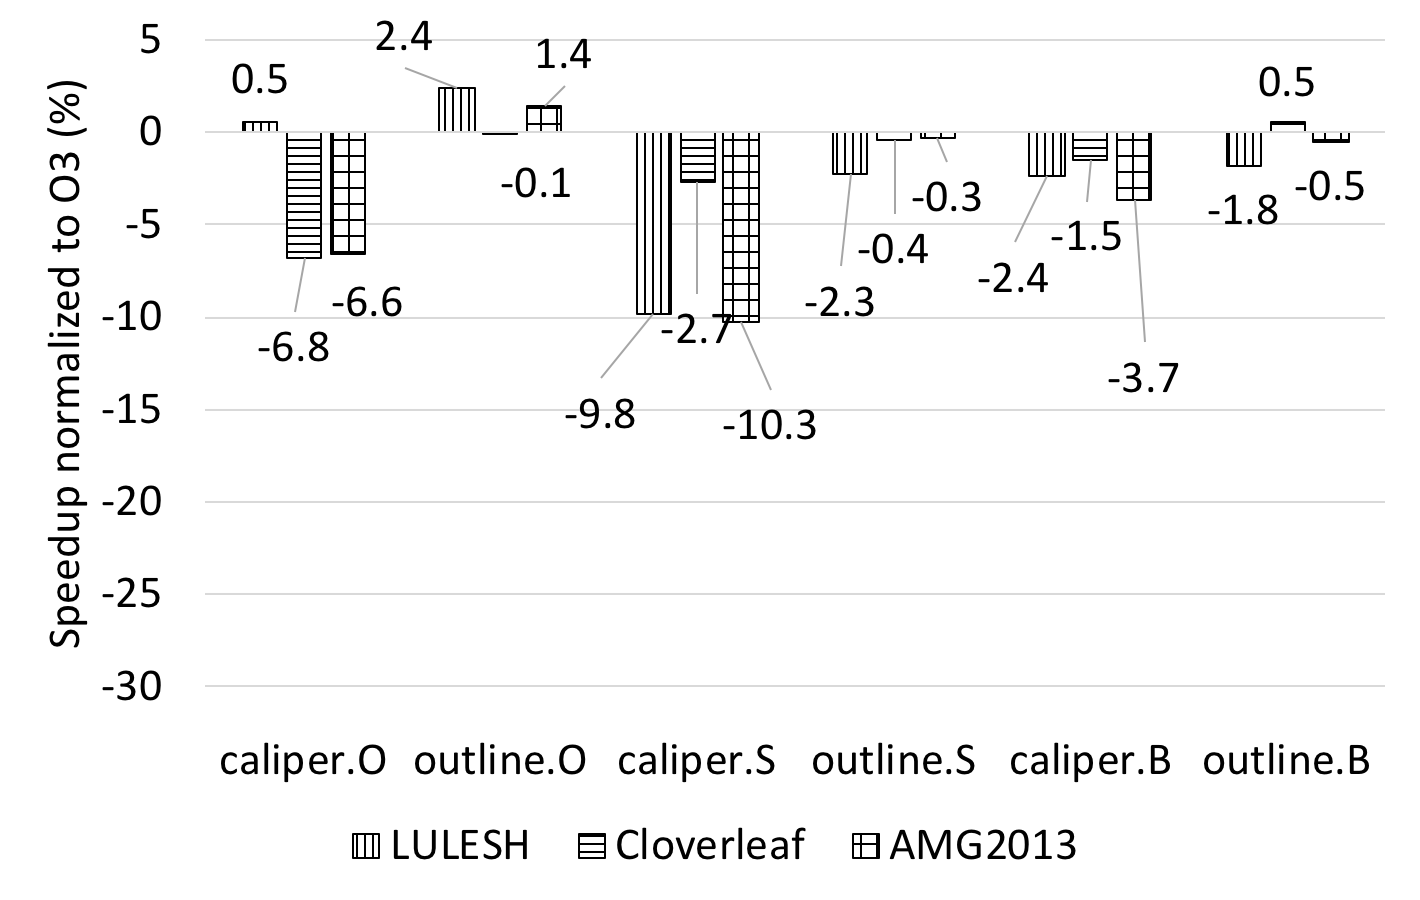
\includegraphics[width=\linewidth]{figures/overhead_all}
%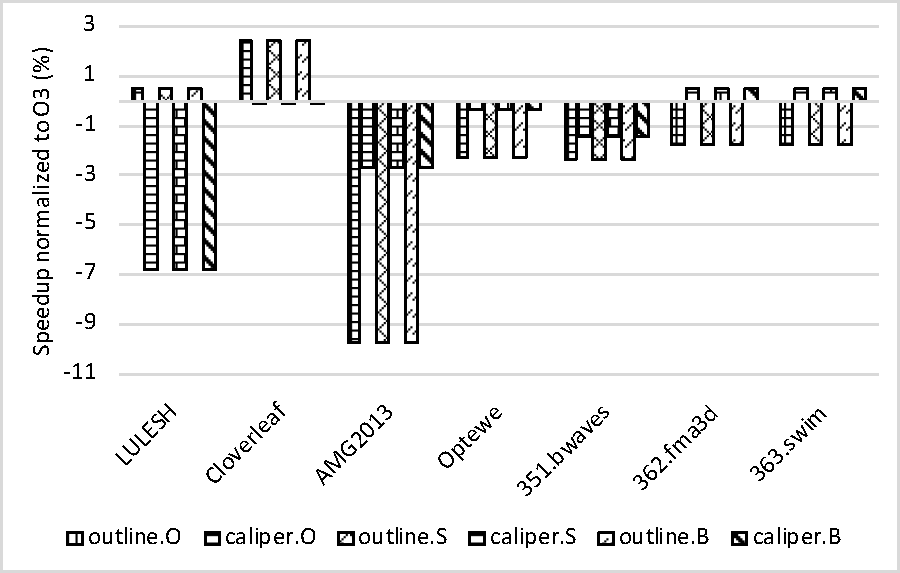
\includegraphics[width=\linewidth]{figures/overhead}
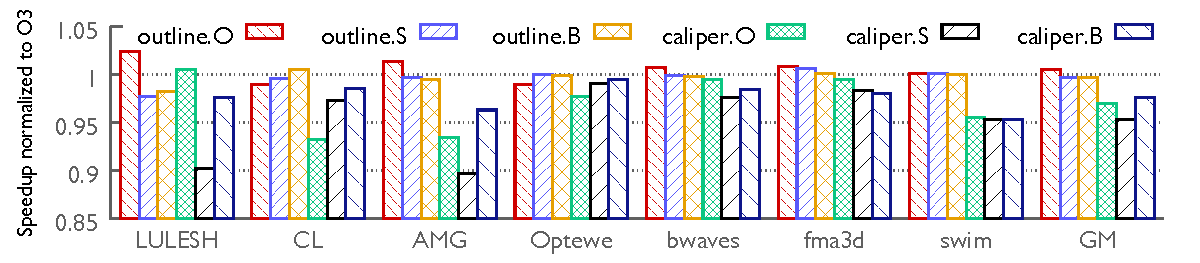
\includegraphics[width=\linewidth]
{gnuplot_temp/overheads.pdf}
\caption{Overheads of loop outlining and Caliper instrumentation on Opteron
  (O), Sandy Bridge (S), and Broadwell (B): outlining results in minimal
  overheads (up to 3\%), but instrumentation can cause noticeable impact.}
\label{fig:overhead}
\end{figure*}

\end{comment}

\subsection{Compiler Flag Selection}

We experiment with 33 optimization-related compilation
flags of the Intel compiler~\cite{icc17manual}.  For flags that
support any value in a continuous range as input, we discretize the
values in the given range.  Then, for each flag $F_i$, \toolname
selects a value $f_i$ from $f_{i1}, f_{i2}, ..., f_{i{n_i}}$ with
equal probability.  A $CV$ is constructed by concatenating the
selected values for all $F_i$s~\cite{opentuner}.  We had to consider
several restrictions when selecting the flags.  First, a flag must not
prevent a program from running successfully on a given target
architecture.  For example, use of the {\em fpack} flag generates code
variants that cause a segmentation fault at runtime and thus {\em fpack } is
excluded.  Second, for fair performance comparison among different
code variants, \toolname enforces strict floating point
reproducibility by discarding floating point related optimization
flags, and always uses {\em -fp-model source } in the presented results.  Last,
optimized library options, such as Intel MKL and IPP
related linkage options, are also excluded since they are not used by
our benchmarks.

Also, in order to reach the full optimization potential of the Intel
compiler tool chain, according to the Intel optimization
note~\cite{iccOpt}, Intel's linker xild and library archive tool xiar
should be used.  We thus modify build systems of all benchmarks
accordingly.
%to meet these practical standards.
Processor-specific flags are also considered for best performance on
each architecture.

\begin{comment}
\begin {table}
%\nocaptionrule
\caption{Notations for code variants. \emph{original}: the unmodified source code; \emph{outlined}: code with hot loops outlined; \emph{caliper}: code with Caliper instrumentation calls; \emph{O3}: the code is compiled with O3 baseline CV.} \label{table:algs}
%\vspace{2pt}
\centering
\begin{tabular}{ l|l }
%\hline
%  & \\
\textbf{Notation} &  \textbf{Definition} \\
\hline
$O3$ &O3, original\\
\hline
$O3.outlined$ &O3, outlined\\
\hline
$O3.caliper$ &O3, outlined and instrumented\\
\hline
$R$ & R, original\\
\hline
\multirow{3}{*}{$G.expected$}
 & Expected runtime of Greedy algorithm.\\
 & $T_{G.expected}=\sum\limits_{j=1}^{J} T_{j{k_j}}$, and\\
 & $k_j=\operatorname*{argmin}_k {\{T_{jk} | 1\leq{k}\leq{K}\}}$\\
\hline
$G.realized$ & Greedy algorithm, outlined\\
\hline
$FR$ &FR, outlined\\
\hline
$Overall$ & CFR, outlined, non-loop code $CV$s with \\
& top-30 lowest end-to-end runtime $T_k$\\
\hline
$Nonloop$ & CFR, outlined, non-loop code $CV$s with \\
& top-30 lowest non-loop code runtime\\
\hline
$Merged$ & CFR, outlined, non-loop code $CV$s \\
&from CFR Overall and Nonloop\\
\hline
$CFR$ & same as CFR merged\\
\hline
\end{tabular}
\end {table}
\end{comment}
% Experimental configurations
\begin{table}[t]
\centering
\caption{Platform overview, runtime configurations, and benchmark inputs.}
%\vspace{-3mm}
%Intel Xeon Phi is configured as Quadrant-Cache mode w/ 16GB MC-DRAM as LLC, which is fastest for our benchmarks.}
\label{settings}
%\bigskip
{
\footnotesize
\begin{tabular}{ p{6.1cm}p{2.2cm}p{2.8cm}p{2.5cm} }
\specialrule{.2em}{.1em}{.1em}
\bf{Machine} &AMD Opteron & Intel Sandy Bridge & Intel Broadwell \\
\hline
\bf{Processor} & Opteron 6128 & Xeon E5-2650 0 & Xeon E5-2620 v4\\
\bf{Sockets} & 2 & 2 & 2 \\
\bf{NUMA nodes} & 4 & 2 & 2  \\
\bf {Cores/Socket} & 4 & 8 & 8  \\
\bf{Threads/Core} & 2 & 2 & 2 \\
\bf{Core Frequency [GHz]} & 2.0 & 2.0 & 2.1  \\
\bf{processor-specific flag} & default & -xAVX & -xCORE-AVX2 \\
\bf{Memory size [GB]} & 32 & 16 & 64\\
\bf{OpenMP thread count} & 16 & 16 & 16\\
\bf{OpenMP thread proclist} & [0-15] & [0-15] & [0-31:2] \\
\bf {LULESH: input size, time-steps} & 120, 10 & 150, 10 & 200, 10 \\
\bf {Cloverleaf: input size, time-steps} & 2000,30 & 2000,30 & 2000,60 \\
\bf {AMG: input size} & 18 & 20 & 25 \\
\bf {Optewe: input size, time-steps} & 320, 5 & 384, 5 & 512, 5 \\
\bf {bwaves: input, time-steps} & train, 10 & train, 15 & train, 50 \\
\bf {fma3d: input} & train & train & train \\
\bf {swim: input} & train & train & train \\
\specialrule{.2em}{.1em}{.1em}
\end{tabular}
}
\vspace{-2mm}
\end{table}

\subsection{Loop Outlining and Caliper Instrumentation}

In order to find code regions that need to be outlined, i.e., separated
into individual modules, \toolname profiles the target application
compiled with ``-O3 -qopenmp -fp-model source''  to identify hot loops.  The profiling is done using
Caliper's instrumentation API~\cite{caliper}, which returns the
per-loop runtime. Only loops whose runtime is at the least 1.0\% of
the baseline's end-to-end runtime, are outlined as independent
compilation modules. Runtime for code other than the hot loops
(non-loop code) cannot be directly measured because such code tend
to be scattered across many source files.  Thus, non-loop code runtime
is derived by subtracting the aggregate runtime of hot loops from
program end-to-end runtime for a given code variant.
%
Caliper instrumentations generally introduce less than 3\% overhead
and the per-loop runtimes are sufficiently informative to \toolname
so that measurement noise is tolerated with its search
algorithms.
%All code variants used in our experiments are listed in
%\Cref{table:algs}.
To evaluate performance, we use ``-O3 -qopenmp -fp-model source'' CV  as
the baseline and report speedup relative to this
baseline unless otherwise specified.  We also note that data points marked {\em
G.expected} are calculated by summing up the best per-loop and non-loop
code runtimes obtained with different compiler options.
%
They are used as an estimation of the upper bound for the Greedy
algorithm. However, this is a hypothetical bound assuming pairwise
independence among different compilation modules. The bound serves as
a reference to assess this independence assumption.

